\chapter{Evalución Continua 3}
\newpage
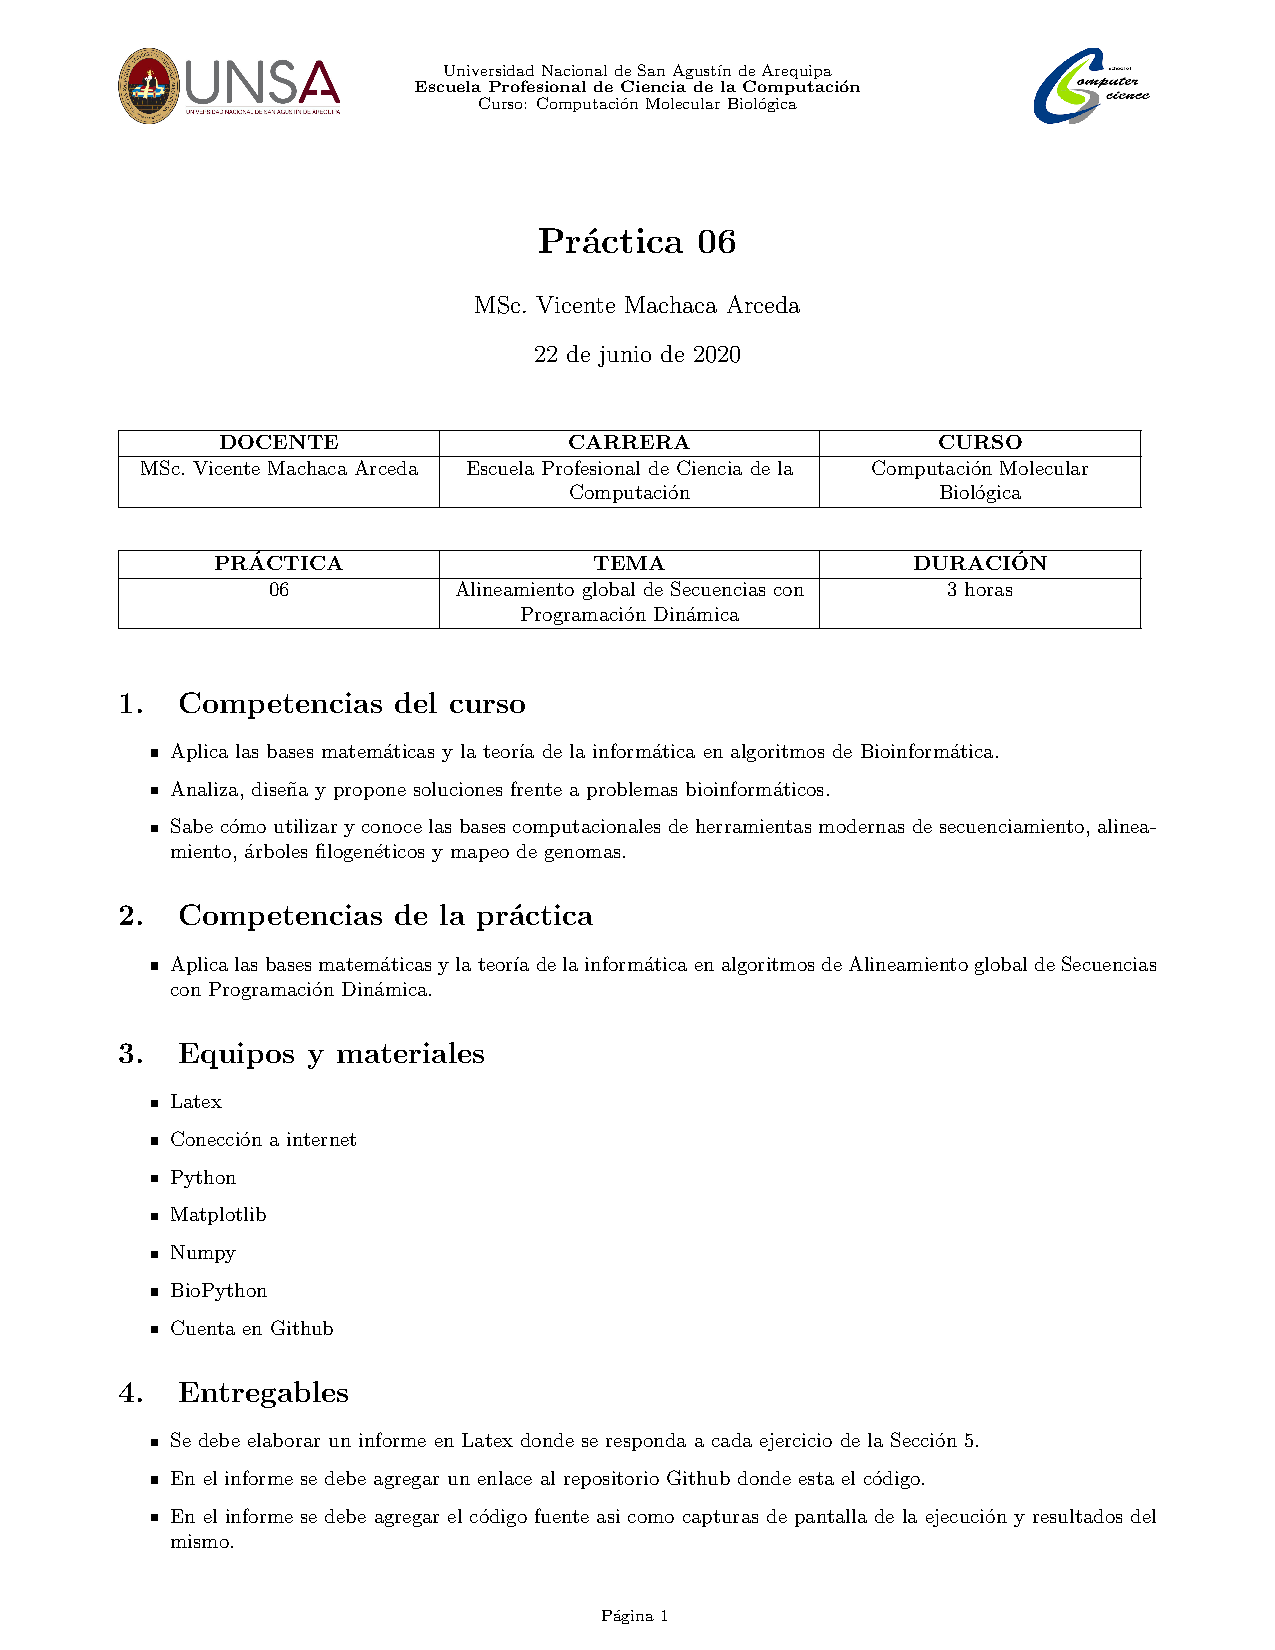
\includepdf[pages={1-}]{pdfs/practices/6_global_alignment.pdf}
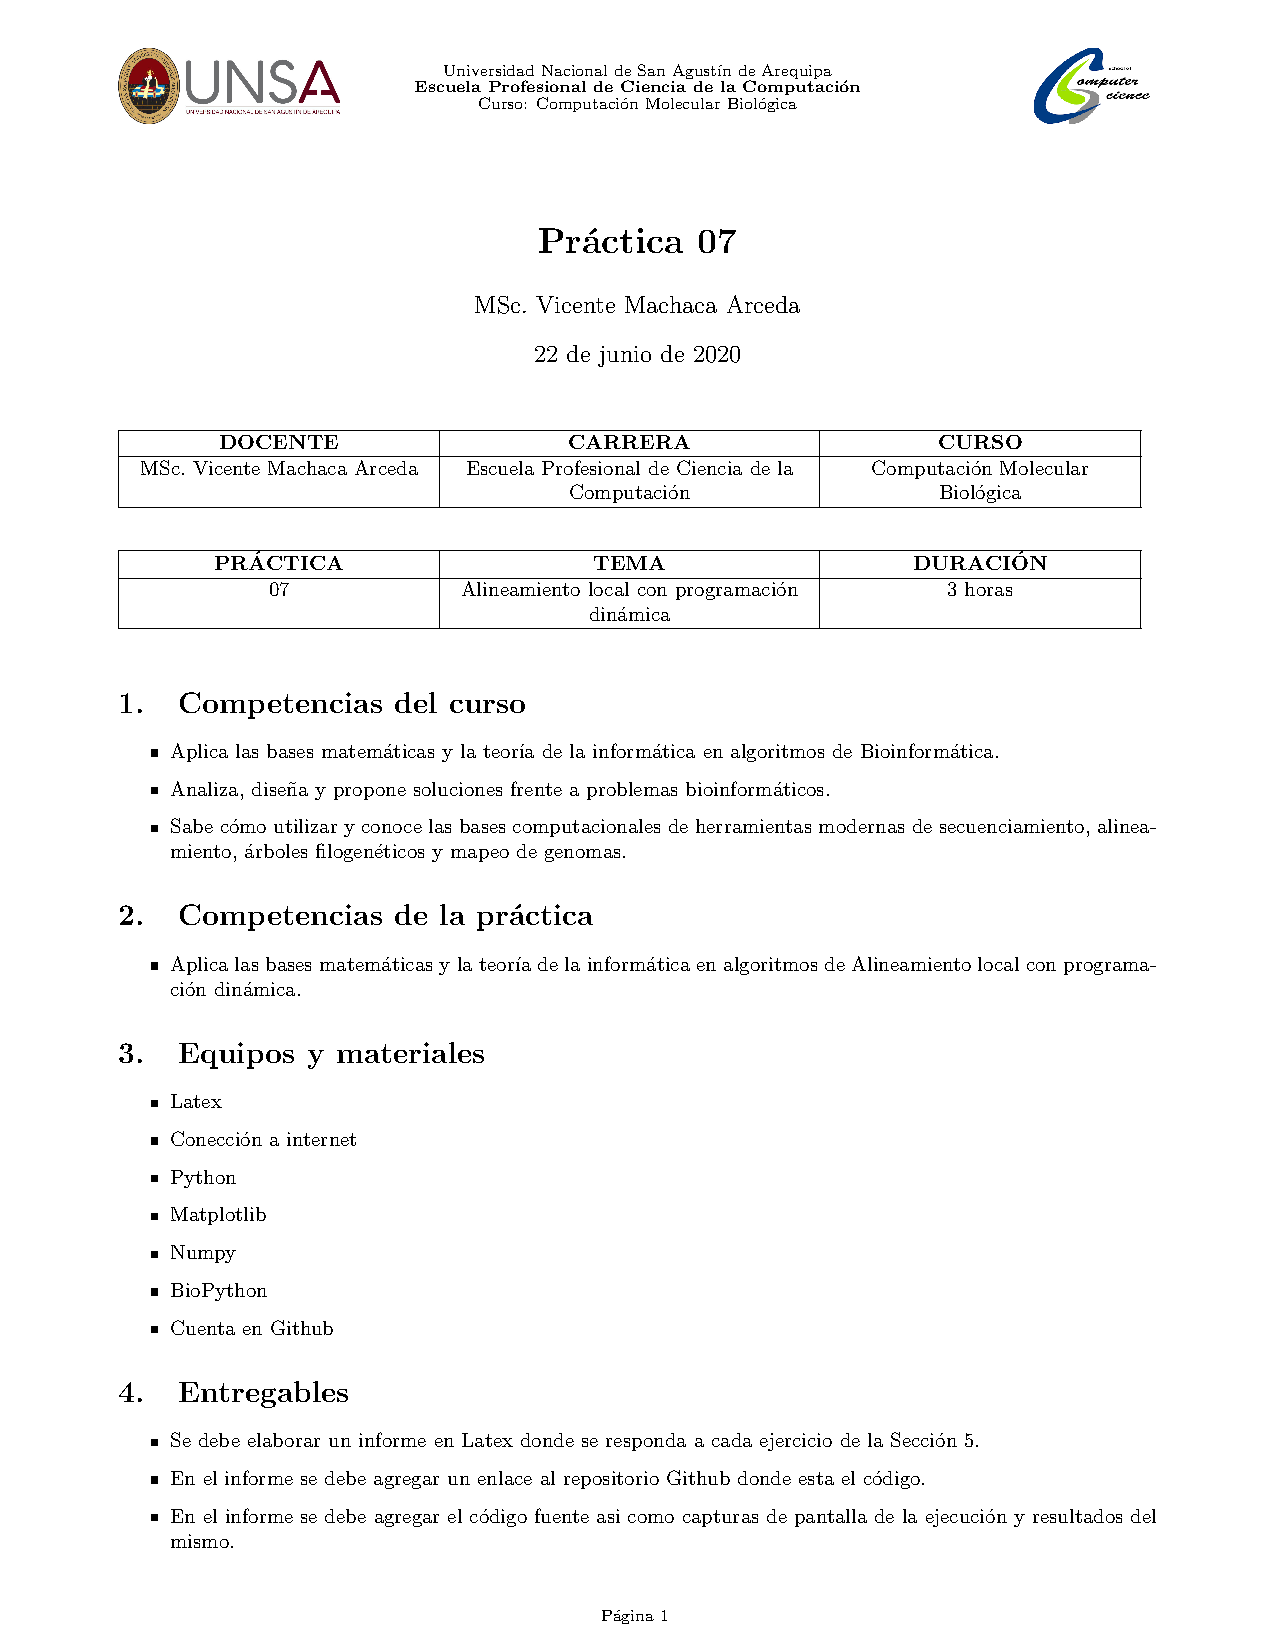
\includepdf[pages={1-}]{pdfs/practices/7_local_alignment.pdf}

\pagestyle{empty} % Disable headers and footers for the following pages

\section{Evidencias}
La evidencia de los Laboratorios realizados por los estudiantes en la Evaluación Continua 3 se muestran en la siguiente tabla:

\begin{table}[h]
\centering
\begin{tabular}{l|c}
\hline
\textbf{Laboratorio} & 
\textbf{Evidencia} 
\\ \hline
Laboratorio 6 &
\href{https://drive.google.com/drive/folders/1uoms3Sf82lClrYDLxP1Al8PQAyQCmEuC?usp=sharing}{Link}
\\ \hline
Laboratorio 7 &
\href{https://drive.google.com/drive/folders/1k54LTmGwlU7G_YXNRZkMFTmEdzDkDSdW?usp=sharing}{Link}
\\ \hline
\end{tabular}
\caption{Evidencia Evaluación Continua 3}
\label{tab:evidencia_evaluacion_continua_3} % Unique label used for referencing the table in-text
%\addcontentsline{toc}{table}{Table \ref{tab:example}} % Uncomment to add the table to the table of contents
\end{table}
%------------------------------------------------


